\documentclass{article}
\usepackage[utf8]{inputenc}
\usepackage[T1]{fontenc}
\usepackage{graphicx}
\usepackage{geometry}
\geometry{a4paper}
\usepackage[frenchb]{babel}
\usepackage{mathtools}
\usepackage{braket}
\title{Brief Introduction to trap-loss atomic collisions}
\author{Xiaoyu Jiang}
\date{12/16/2017}
\begin{document}
\maketitle
\section{General Introduction}
Atomic collisions plays a key role in many branches of modern physics research. The basic reason for studying it is that collisions gives us information on the atoms involved in the collisions if the interactions between them are already well-understood, or vice versa. It also gives experimentalists a powerful tool tool to manipulate atoms, which is particularly important in cold atoms physics. 

Atomic collsions theory is a very broad and fruitful part of atomic physics. Many factors such as temperature, atomic states, and external potentials could all have influences on the dynamics of collisions, thus leading to phenomenons like state-change, temperature shift, ionization, etc. We would first give a very brief review of quantum scattering theory, which is the most elementary tool for studying collisions. Then we will foucus on discussing a particular topic in atomic collisions: collisions that lead to trap losses.

Part 2 of this paper mainly follows \emph{Principles of Quantum Mechanics} by Shankar and the notes of Physics 732 by Prof. Everett. Part 3 is written mainly based on \emph{Experiments and Theory in Cold and Ultracold Collisions}, a review paper by Weiner et al on 1999. 

\section{Review of quantum scattering theory}
Let's first consider a case where two atoms(or particles) with the same mass $m_1$ and $m_2$ collide with each other. Let $V$ be the interaction potential between the atoms. To make the case simple we first neglect the internal structure of the atoms, then the Hamiltonian of the system becomes: 
$$ \hat{H}=\frac{\hat{p_1}^2}{2m_1}+\frac{\hat{p_2}^2}{2m_2}+V(\hat{\vec{r_1}}-\hat{\vec{r_2}}) $$
which can be written as
$$ \hat{H}=\frac{\hat{P_{CM}}^2}{2M}+\frac{\hat{p_{r}}^2}{2m_{r}}+V(\hat{\vec{r_{r}}}) $$
In which $P_{CM}$ and $M$ are the mometum and mass of the center-of-mass of the system, $p_r$, $m_r$ and $r_r$ are the relative variables. We are interested in the relative motion between the atoms, so the problem can be taken as an incident particle with momentum $p_{r}$ scattering on the potential $V(r_{r})$. The solution of Shrodinger Equation:
$$ (\frac{\hat{p_{r}}^2}{2m_{r}}+V(\hat{\vec{r_{r}}}))\psi_k(\vec{r})=E_k\psi_k(\vec{r})$$ 
will have the follwing asymptotic form:
$$\psi_k(r){~}e^{ikz}+f(\theta,\phi)\frac{e^{ik\vec{r}}}{r}$$
under the condition that $V(r)$ goes to zero when $|r|$ goes to infinity, and $r\gg b$, where $b$ is the effective range of the potential, and $z$ is the axis along the direction of incidation. From here on we will drop all the subscripts on the relative variables. The solution shows that the wavefunction is a combination of incident wave and scattered wave, when the incident wave is a plane wave with momentum $k$. $f(\theta,\phi)$ is called the scattering amplitude. 

One interesting quantity would be the differential cross section, which is defined as the ratio between number of particles scattered into $d\Omega$ per unit time and the incident flux. Further evaluation shows:
$$\frac{d\sigma}{d\Omega}d\Omega=|f(\theta,\phi)|^2$$
The total cross section $\sigma$ is the ratio between the total number of scattered particles and the incident flux, which is jut the integral of  :
$$\sigma=\int{\frac{d\sigma}{d\Omega}d\Omega}$$
Our task now is to solve for the scattering amplitude $f(\theta,\phi)$.
\subsection{Partial wave expansion}
 If we consider a spherically symmetric potential $V(\vec{r})=V(r)$, then $[\hat{H},\hat{L_z}]=0$. The incoming plane wave can be expanded by Legendre polynomials:
$$e^{ikz}=e^{ikr\cos{\theta}}=\sum_{l}i^l(2l+1)j_l(kr)P_l(\cos{\theta})$$
Then we can also solve for $f(\theta)$ and expand it. Here $f$ only depends on $\theta$ because of the symmetry of the potential. Calculation shows that it takes the form:
$$f(\theta)=\frac{1}{k}\sum_{l}(2l+1)e^{i\delta_l}\sin{\delta_l}P_l(\cos{\theta})$$
Here $\delta_l$ the phase shift added to each $l$ componet of the incident wave. It depends on the incident momentum $k$ and the exact potential $V(r)$. We still need to solve the radial Schrodinger equation to find it, but it at least it has some physical meaning to the real experiments and measurements. 

\section{Study of trap-loss atomic collisions}
In the introduction above we have been studying collisions between simple particles that has no internal structures. However, most atoms would have nonzero internal angular momentum even at ground states considering fine and hyperfine structures. Thus besides considering the change of spatial wave functions, one also needs to take into account the possible state-change of the participating atoms. Let $a$, $b$ be the two atoms involved, $\ket{a_ib_i}$ be the initial state and $\ket{a_fb_f}$ be the final state, we can divide the collisions into two categories: elastic and inelastic. 

For elastic collisions, $\ket{a_ib_i}=\ket{a_fb_f}$, indicating that the internal states of atoms $a$ and $b$ was not changed. For trapped atoms, which are what we are interested in, elastic collisions only exchages momentum between atoms and won't cause any additional heating to the trapped atomic cloud, thus does not contribute to any significant trap loss. 

For inelastic collisions, $\ket{a_ib_i}\neq\ket{a_fb_f}$. In the case where $\Delta{E}=E_f-E_i<0$, the differece of internal energy$\Delta{E}$ will then become part of the spatial kinetic energy of the system, causing the temperature of the atomic cloud to rise and degrades the efficiency of trapping. For atoms trapped by lasers the following figure for potential energy shows some key features of this collision process:

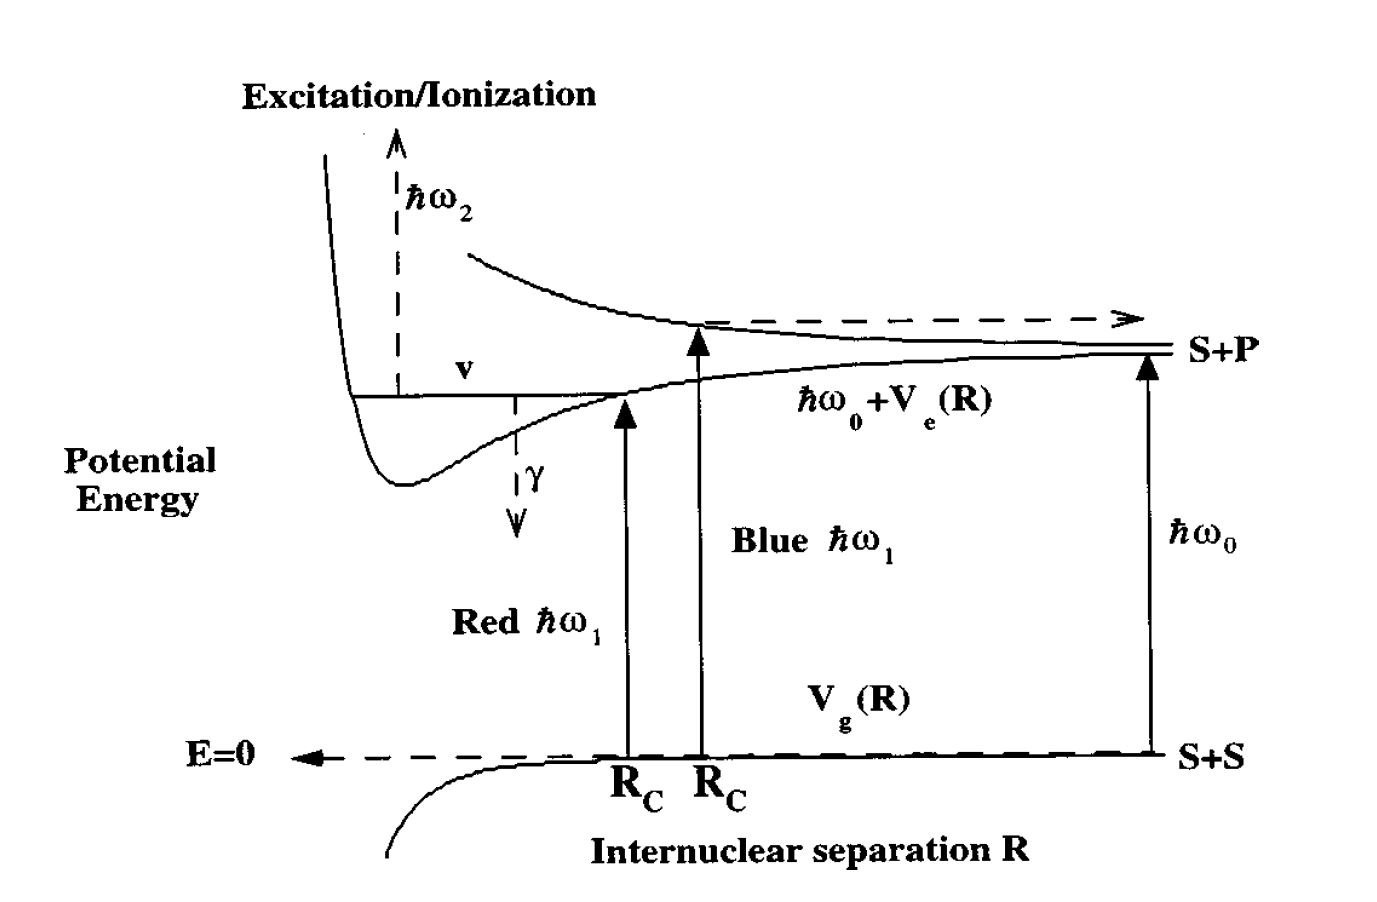
\includegraphics[height=3in]{collisions.JPG}

In this figure the S+S curves correspond to the interaction energy between two ground state atoms, which at long range has an asymptotic form of ${C_6}/{R^6}$. The two S+P curves correspond to the potential energy between a ground state S atom and an optically excited P atom. The potential is generated by diople-diople interactions and has a form of $\pm{C_3}/{R^3}$. Here $C_6$ and $C_3$ are all constants. 

The basic idea is that at the initial stage of collsions one of the atoms absorbs a photon from a trapping beam and gets excited from S state to P state.  We would assume the intercating S and P atoms forms a quasi-molecule, and the curves on the diagram is the potential energy of the system. After forming a quasi-molecule, the state of the system would move along the curves to a lower potential. The length of this process can be taken as the time passed during the collision. For attactive potentials, during the collision time, there are possibilities that the excited atom would emit a red-shifted photon and goes back to ground state.  The excess energy would then add to the kinetic energy of the system and heat the atoms. This process is named as radiactive escape. 

The Condon point $R_C$ is defined as a particular distance between atoms where the potential difference between S+P state and S+S state matchs the energy of incident photon.


There are also other reasons for a collision in this model to be inelastic. Considering that the excited state of the atom could be non-degenerate, the collision process could, instead of restoring the excited atom back to ground state,  result leaving the excited atom in a different fine structure state or hyperfine structure state. The difference in the energy can then contribute to the kinetic energy of the system. For alkali atoms the change of fine structure states is anoter major reason for inelastic collisions.



\subsection{Gllagpher-Pritchard model}
Gllagpher and Pritchard proposed a semiclassical model in 1989 to describe the radiactive and fine-structure changing inelastic collisions for trapped alkali atoms. It gives a clear physics picture for people to understand collision dynamics. The follwoing figure shows the key features for this case:

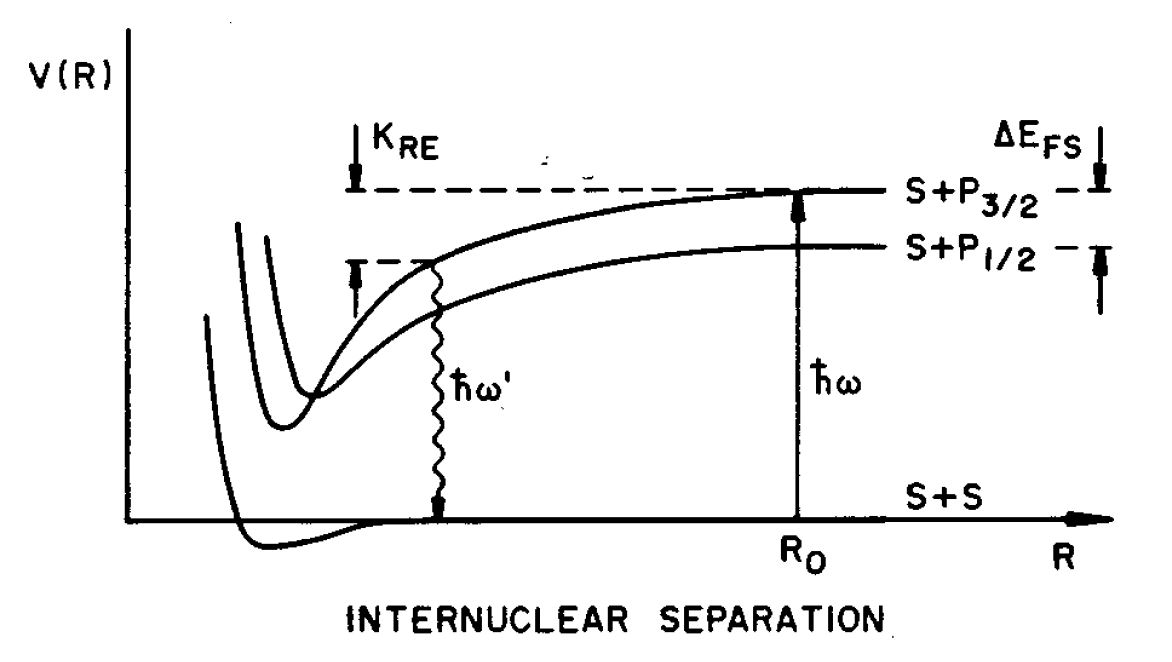
\includegraphics[height=3in]{G-P.JPG}

In this figure the inelastic collisions starts when one atom gets excited by absorbing a phonton with frequency $\omega$. Then as a quasi-molecue the system slides to shorter internuclear seperations. During this process, radiactive escape happens when the excited atom spotaneously decays back to ground state and emits a photon with frequency $\omega^{'}$, which is red detuned compared to $\omega$. When spontaneous emission does not happen, the state of the system could be changed from $S+P_{3/2}$ to $S+P_{1/2}$, because the corresponding potential curve of these two states would cross at some point, when the two atoms gets closer. 

For radiative escape we can describe the system by writing:
$$A+A+\hbar\omega\rightarrow{A_2^*}\rightarrow{A+A+\hbar\omega^{'}}$$

For fine structure changing collisions(FCC) we can write:
$$A+A+\hbar\omega\rightarrow{A_2(P_{3/2})^*}\rightarrow{A_2(P_{1/2}^*)+\Delta{E_{FS}}}$$.

The inelastic collision starts by exciting two ground-state atoms to a quasi-molecular level. The rate of this excitatiion is given by:
$$R(R_0,\omega,I)=[\frac{(\gamma/2)^2}{(\gamma/2)^2+\Delta^2}]\frac{I}{\hbar\omega}\frac{\lambda^2}{2\pi}$$

Here $\Delta=\omega-\omega_{R_0}$, and $\omega_{R_0}=\omega_A-C_3/(\hbar R_0^3)$, and $\omega_A$ is the atomic resonant fequency. $\lambda^2/2\pi$ is the photon-absorption cross section to attractive molecular states. $I$ is the intensity of the laser. $\gamma$ is the molecular spontaneous decay rate. 

The time that takes the molecule to reach the bottom of the potential is approximately the same as the time that it takes to get to $R=0$. The time can be calculated by integrating the equation of motion:
$$t(R_0)=(\frac{M}{4})^{1/2}\int_0^{R_0}dR(\frac{C_3}{R^3}-\frac{C_3}{R_0^3})^(-1/2)$$

which finally gets to:
$$t(R_0)=0.747(\frac{MR_0^5}{4C_3})^{1/2}$$

where $M$ is the atomic mass. Then the probability of not having a spontaneous emission is:
$$\eta=e^{-\gamma{t(R_0)}}$$

For the molecule oscillating repeatedly in the potential, the total probability for FCC would then be:
$$P_{FCC}=\zeta\eta+\zeta(1-\zeta)\eta^3+...=\frac{\zeta\eta}{[1-\eta^2+\zeta\eta^2]}$$

Here $\zeta$ is the probability of FCC in a signle oscillation. $\zeta=2P(1-P)$, where P is the Landau Zener single-transit curve-crossing probability. 

The total rate of FCC is then the integral over all possible $R_0$s. Let $n$ be the atomic density in the trap, then the number of pairs within seperation $R_0\rightarrow R_0+dR$ would be $n^24\pi R_0^2dR_0/2$. Integrate over $R_0$, we get the rate of FCC:
$$R_{FCC}=\frac{n^2}{2}\int_0^\infty dR_04\pi R_0^2R(R_0,\omega,I)P_{FCC}(R_0)$$
 
We can follow the same process for radiative escape collisions. Define $R_E$ such that for $R_0<R_E$, the kinetic energy received by atoms will be sufficient for trap-escaping. The total probabilty would be in the same form as $P_FCC$, except that we need to change $\zeta$ to $2\gamma t_E(R_0)$, which is the probability for spontaneous emission when $R_0<R_E$:
$$P_{RE}(R_0)=\frac{2t_E(R_0)\gamma\eta}{[1-\eta^2+\zeta\eta^2]}$$

The total rate would then be:
$$R_{RE}=\frac{n^2}{2}\int_0^{R_E} dR_04\pi R_0^2R(R_0,\omega,I)P_{RE}(R_0)$$

\subsection{Assesment of G-P model}
The Gllagpher-Pritchard model provides us with a semi-classical way of understanding trap-loss atomic collisions qualitatively. Besides G-P model there has been many other semi-classical or quantum models of explaning and studying atomic collisions in traps.

For small detunings(compared to the order of 10 atomic line widths), we still haven't found a theory that can explain the collision dynamics quantitatively.  Becasue of the small detuning, the Condon point $R_C$ becomes large, and it leads to two major problems. First is that large $R_c$ means that it takes a very long time for the atom to travel from where they got excited to small $R$ values. As a result the spontaneous decay would have a very high weight compared to FCCs. Large $R_C$ also means that the majority of the molecular potential is flat, and the complex structure of the molecular hyperfine structure would have a considerable shift on the potential. This makes the calculation for $t(R_0)$ in the previous section invalid. 

The G-P model works very well at large detunings, due to the fact that the Condon point $R_C$ is sufficiently small for small detunings. This allows us to neglect molecular hyperfine energy levels because of the steep attractive potentials. Theoretical calculations shows nice agreement with experimets. \newline\newline\newline
\newline
\textbf{References}\newline
1. Notes of Physics 732, Prof Everett, UW-Madison,2017.\newline
2. Notes of Physics 545, Prof Saffman, UW-Madison2017.\newline
3. Shankar, Ramamurti. Principles of quantum mechanics. Springer Science \& Business Media, 2012.\newline
4. Weiner, John, et al. "Experiments and theory in cold and ultracold collisions." Reviews of Modern Physics 71.1 (1999): 1.\newline
5. Dalibard, Jean. "Collisional dynamics of ultra-cold atomic gases." Proceedings of the International School of Physics-Enrico Fermi. Vol. 321. 1999.\newline
6. Gallagher, Alan, and David E. Pritchard. "Exoergic collisions of cold Na-Na." Physical review letters 63.9 (1989): 957.\newline
7. Woodgate, Gordon Kemble. "ELEMENTARY ATOMIC STRUCTURE." (1970).\newline
8. Weidemueller, Matthias, and Claus Zimmermann. "Cold atoms and molecules. A testground for fundamental many particle physics." (2009).\newline
9. Suominen, K-A., et al. "Quantum and semiclassical calculations of cold-atom collisions in light fields." Physical Review A 57.5 (1998): 3724.\newline




\end{document}

%------------------------------------------------------------------------------------------------------------------